%% Submissions for peer-review must enable line-numbering
%% using the lineno option in the \documentclass command.
%%
%% Preprints and camera-ready submissions do not need
%% line numbers, and should have this option removed.
%%
%% Please note that the line numbering option requires
%% version 1.1 or newer of the wlpeerj.cls file, and
%% the corresponding author info requires v1.2

\documentclass[fleqn,10pt,lineno]{wlpeerj} % for journal submissions
% \documentclass[fleqn,10pt]{wlpeerj} % for preprint submissions
\usepackage{textcomp} %for \textgreater
\usepackage{wasysym} %for \times
\usepackage{hyperref}

\title{Patterned progression of gut microbiota predisposes preterm infants to necrotizing enterocolitis and late onset sepsis: pilot data from a non-Western population}

\author[1]{Jiayi Liu}
\author[2]{Jianhua Sun}
\author[3]{Yuqing Li}
\author[4]{Yi Feng}
\author[5]{Liya Pan}
\author[6]{Zhoulonglong Xie}
\author[7]{Zhilong Yan}
\author[8]{Jianhua Zhao}
\author[9]{Li Hong}


\affil[1]{Department of Clinical Nutrition, Shanghai Children's Medical Center, School of Medicine Shanghai Jiao Tong University, Shanghai, China}
\affil[2]{Department of Clinical Nutrition, Shanghai Children's Medical Center, School of Medicine Shanghai Jiao Tong University, Shanghai, China}
\affil[3]{Department of Clinical Nutrition, Shanghai Children's Medical Center, School of Medicine Shanghai Jiao Tong University, Shanghai, China}
\affil[4]{Department of Clinical Nutrition, Shanghai Children's Medical Center, School of Medicine Shanghai Jiao Tong University, Shanghai, China}
\affil[5]{Department of Clinical Nutrition, Shanghai Children's Medical Center, School of Medicine Shanghai Jiao Tong University, Shanghai, China}
\affil[6]{Department of Clinical Nutrition, Shanghai Children's Medical Center, School of Medicine Shanghai Jiao Tong University, Shanghai, China}
\affil[7]{Department of Clinical Nutrition, Shanghai Children's Medical Center, School of Medicine Shanghai Jiao Tong University, Shanghai, China}
\affil[8]{Shanghai Majorbio Bio-Pharm Technology Co., Ltd, Shanghai, China}
\affil[9]{Department of Clinical Nutrition, Shanghai Children's Medical Center, School of Medicine Shanghai Jiao Tong University, Shanghai, China}
\corrauthor[9]{Li Hong}{hongli@scmc.com.cn}

%\keywords{Gut Microbiota, Preterm Infant, Necrotizing Enterocolitis, Neonatal Late Onset Sepsis, High Throughput DNA Sequencing, DADA2}

\begin{abstract}
\textbf{Background and Objectives} \\Intestinal microbiota dysbiosis might predispose preterm infants to necrotizing enterocolitis(NEC) and late onset sepsis(LOS). In this observational prospective study, we aimed to profile and compare postpartum microbiota progression patterns in non-Western preterm patients with either condition. \\
\textbf{Methods} \\We enrolled preterm infants with gestational age less than 33 weeks and birth weight more than 950g, from July 2013 to December 2014. We began fecal sample collection from the the first stool after birth and prospectively collected until discharge. Bacterial V3~V4 region of 16s rRNA genes from each stool sample were amplified, sequenced and analyzed. \\
\textbf{Results}\\A total of 192 fecal samples from 24 patiens were studied, of whom four developed NEC, three LOS; the remaining 17 were used as controls. [The post-partum gut microbiota colonization started to diverge among NEC, LOS and their matched control groups, from the second week after birth.  Microbiota of the LOS infants was the least diversified (Shannon index=1.66), while that of the control group was the most diversified(Shannon index=0.88, p=0.01). Potentially pathogenic genus Enterococcus (20.86\%) and Staphylococcus (8.67\%) were prominent in NEC patients and Klebsiella (42.15\%) in LOS group. Both two groups addressed lower proportion of Lactococcus (7.98\% and 13.76\% in NEC and LOS group, respectively) than the control group (3.66\%)].\\
\textbf{Conclusions}\\Postpartum colonization pattern of gut microbiome might predispose preterm newborns to NEC or LOS, in which reduced diversity of the whole microbiota community and potentially pathogenic genus could have played an essential role in disease progression. Still, more studies are needed to identify etiological strains, underlying mechanisms and correspondent microbial patterns.
\end{abstract}

\begin{document}

\flushbottom
\maketitle
\thispagestyle{empty}

\section*{Introduction}
Gut microbiota is a key contributor to human health and the dysbiosis of which are proven to be associated with diseases, such as atherosclerosis\citep{tang2017gut}, obesity\citep{bouter2017role}, neuropathy\citep{sarkar2016psychobiotics}, liver diseases\citep{tilg2016gut}, etc. Temporal colonization pattern of the intestinal microbiota during early stages of life\cite{} also provided evidence of its association with early life events, including Type 1 diabetes\citep{giongo2011toward, vatanen2018human}, asthma\citep{stokholm2018maturation} and allergy\citep{madan2012normal,savage2018prospective}. In light of interindividual variability in gut maturity, innate immunity, birth mode and enviromental exposures, preterm infants are predisposed to complications post-partum intestinal microbiota development

\noindent
In preterm infants, necrotizing enterocolitis and late onset sepsis

\noindent
Necrotizing enterocolitis, characterized by rapid progression, high morbidity and mortality, is one of the most devastating gestrointestinal neonatal emergencies, especially in preterm newborns. Previous studies have suggested well how intestinal microbiota pattern is implicated prior to, during and after the course of this condition. Mai et al. reported an increase in the Proteobacteria and a decrease in the Firmicutes phyla during three to seven days prior to NEC onset (Mai et al., 2011). Zhou et al. found a relatively higher abundance of Clostridium and Gamma-Proteobacteria in the proximity of NEC during early and late onset, respectively (Zhou et al., 2015).

late onset sepsis is

 Among non-Western population, however, evidence (few studies on?) of microbiota chronological dysbiosis preceding necrotizing enterocolitis or late onset sepsis has been scant so far. Hence, conducting a prospective study among Chinese patients using high-throughput DNA sequencing, we aimed to profile and compare post-postpartum pattern of intestinal microbiota in preterm infants who subsequently developed necrotizing enterocolitis and late onset sepsis, which may be critical in the etiopathogenesis of disease.

\section*{Methods}
  \subsection*{Ethics}
  This study was approved by the joint committee of ethics of Shanghai Children’s Medical Center, School of Medicine Shanghai Jiao Tong University (SCMCIRB-K2013022). Detailed written informed consent was obtained from the parents prior to fecal sample collection.

  \subsection*{Patients}
  Newly born preterm infants with gestational age less than 33 weeks, birth weight over 950g were enrolled from Neonatal Intensive Care Unit at Shanghai Children’s Medical Center from July 2013 to December 2014. The exclusion criteria were 1) diagnosed with early-onset sepsis, 2) hepatic diseases, 3) renal impairment (Cr \textgreater 88 $\mu$M), 4) diagnosed with intestinal obstruction, 5) in foreseeable need of cardiovascular or abdominal surgeries (except for male circumcision or PDA ligation), 6) estimated parenteral support to supply over 50\% of daily caloric intake for more than four days, 7) given intravenous antibiotics administration (except prophylactic regimen of cefotaxime, piperacillin-tazobactam and/or metronidazole), 8) history of oral antibiotics administration, 9) grossly bloody stools at admission, and 10) over five days old.

  NEC cases were defined as infants who met the criteria for Stage II and Stage III NEC disgnosis\citep{bell1978neonatal}, including radiographic intestinal dilation, ileus, pneumatosis intestinalis, and/or absent bowel sounds with or without abdominal tenderness, and/or mild metabolic acidosis and thrombocytopenia. LOS cases was diagnosed if 1)an infant had a positive hemoculture or other suspicious loci of infection after 72 hours of life, with septic signs/symptoms reviewed independently by at least two neonatologists, and had been treated with advanced antibiotics (e.g., Meropenem) after diagnosis. Infants with no infectious complications or sepsis were regarded as controls.

  \subsection*{Sample collection and handling}
  Fecal samples collection began from neonatal meconium till discharge.   Although we intended to collect fecal samples on a daily basis, due to working shifts and flexible clinical scheduling, we set seven days as the maximum interval between two collections from every infant. Every sample was collected within 30 minutes of defecation from patients' diaper with a sterile spatula. The samples were immediately placed in a cryogenic vial on dry ice and stored at 80\textdegree{}C within 30 minutes without additives. All samples were collected and stored before knowing the diagnosis of respective patients.

  \subsection*{DNA extraction and quality control amplification and 16s rRNA gene sequencing}
  Microbial genomic DNA was isolated from each fecal specimen using the E.Z.N.A.® Soil DNA Kit (Omega Bio-Tek, Norcross, GA, U.S.) according to manufacturer’s protocols. The concentration and purity of the DNA were determined by NanoDrop 2000 UV-vis spectrophotometer (Thermo Scientific, Wilmington, USA), and the DNA quality was checked by 1\% agarose gel electrophoresis.

  \subsection*{Broad-range PCR and High-throuput Sequencing of 16s rRNA gene amplicons}
  The V3-V4 hypervariable regions of the bacterial 16S rRNA gene were amplified from each sample using bacterialarchaeal primers 338F (5’-ACTCCTACGGGAGGCAGCAG-3’) and 806R (5’-GGACTACHVGG GTWTCTAAT-3’) using thermocycler PCR system (GeneAmp 9700, ABI, USA). The PCR reactions were as follows: 3 min of denaturation at 95 °C, 27 cycles of 30 s at 95 °C, 30 s annealing at 55 °C and 45 s elongation at 72 °C, and a final extension at 72 °C for 10 min. The PCR reactions were performed in triplicate, with each 20 $\mu$L mixture containing 4 $\mu$L 5X FastPfu Buffer, 2 $\mu$L 2.5 mM dNTPs, 0.8 $\mu$L of each primer (5 $\mu$M), 0.4 $\mu$L FastPfu Polymerase and 10 ng template DNA. The PCR products were extracted from a 2\% agarose gel and further purified using the AxyPrep DNA Gel Extraction Kit (Axygen Biosciences, Union City, CA, USA), and quantified using QuantiFluor™-ST (Promega, USA) according to the manufacturer’s protocols.

  Equimolar amounts of purified amplicons were pooled and paired-end sequenced (2 x 300) on an Illumina MiSeq platform (Illumina, San Diego, USA) according to the standard protocols of Majorbio Bio-Pharm Technology Co. Ltd. (Shanghai, China). The reads were de-multiplexed using the Illumina software and separate FASTQ files were generated for each specimen and deposited to the Sequence Read Archive NCBI under the BioProject accession PRJNA470548. Another public archive repository is available at \href{https://figshare.com/articles/Untitled_Item192_samples_for_publishing_Longitudinal_gut_microbiota_patterns_in_preterm_infants_with_necrotizing_enterocolitis_or_late-onset_sepsis_an_observational_prospective_study_/7205102}{figshare doi: 10.6084/m9.figshare.7205102}

  \subsection*{Bacterial Species Classification Reference Set Creation}


  \subsection*{Statistical Analysis}
    \subsubsection{Demographics and Clinical Sample comparisons}
    Non-parametric tests, including Kruskal-Wallis test and Wilcoxon rank-sum test (SPSS Version ???(SPSS Inc. )) were used to compare gestational age, birth weight, age when the patients were diagnosed as NEC or LOS and length of stay at $\alpha$ level of 0.05 among three groups. !!!!SPSS version check!!!Fisher’s exact test
    \subsubsection{Microbiota Analyses}





\section*{Results}
\subsection*{Patients and samples characteristics}

\section*{Discussion}
Previous studies have



\section*{Conclusions}
Necrotizing enterocolitis,  a worldwidely concern that threatern

\section*{Acknowledgments}
We appreciate the support from enrolled patients, their families, and all staffs at Shanghai Children’s Medical Center.


%microbiota development in infancy, sequence effect, Conversely, adequate maturation of the gut microbiome in this period may protect these pre-disposed children.
%increase vulnerability





\section*{Some \LaTeX{} Examples}
\label{sec:examples}

Use section and subsection commands to organize your document. \LaTeX{} handles all the formatting and numbering automatically. Use ref and label commands for cross-references.

\subsection*{Figures and Tables}

Use the table and tabular commands for basic tables --- see Table~\ref{tab:widgets}, for example. You can upload a figure (JPEG, PNG or PDF) using the project menu. To include it in your document, use the includegraphics command as in the code for Figure~\ref{fig:view} below.

\begin{figure}[ht]
\centering

\includegraphics[width=\linewidth]{view.jpg}
\caption{An example image.}
\label{fig:view}
\end{figure}

\begin{table}[ht]
\centering
\begin{tabular}{l|r}
Item & Quantity \\\hline
Widgets & 42 \\
Gadgets & 13
\end{tabular}
\caption{\label{tab:widgets}An example table.}
\end{table}

\subsection*{Citations}

LaTeX formats citations and references automatically using the bibliography records in your .bib file, which you can edit via the project menu. Use the cite command for an inline citation, like \cite{Figueredo:2009dg}, and the citep command for a citation in parentheses \citep{Figueredo:2009dg}.

\subsection*{Mathematics}

\LaTeX{} is great at typesetting mathematics. Let $X_1, X_2, \ldots, X_n$ be a sequence of independent and identically distributed random variables with $\text{E}[X_i] = \mu$ and $\text{Var}[X_i] = \sigma^2 < \infty$, and let
$$S_n = \frac{X_1 + X_2 + \cdots + X_n}{n}
      = \frac{1}{n}\sum_{i}^{n} X_i$$
denote their mean. Then as $n$ approaches infinity, the random variables $\sqrt{n}(S_n - \mu)$ converge in distribution to a normal $\mathcal{N}(0, \sigma^2)$.

\subsection*{Lists}

You can make lists with automatic numbering \dots

\begin{enumerate}[noitemsep]
\item Like this,
\item and like this.
\end{enumerate}
\dots or bullet points \dots
\begin{itemize}[noitemsep]
\item Like this,
\item and like this.
\end{itemize}
\dots or with words and descriptions \dots
\begin{description}
\item[Word] Definition
\item[Concept] Explanation
\item[Idea] Text
\end{description}

We hope you find write\LaTeX\ useful for your PeerJ submission, and please let us know if you have any feedback. Further examples with dummy text are included in the following pages.

\section*{Methods}

\lipsum[4] % Dummy text

\begin{equation}
\cos^3 \theta =\frac{1}{4}\cos\theta+\frac{3}{4}\cos 3\theta
\label{eq:refname2}
\end{equation}

\lipsum[5] % Dummy text

\subsection*{Subsection}

\lipsum[6] % Dummy text

\paragraph{Paragraph} \lipsum[7] % Dummy text
\paragraph{Paragraph} \lipsum[8] % Dummy text

\subsection*{Subsection}

\lipsum[9] % Dummy text

\begin{figure}[ht]\centering
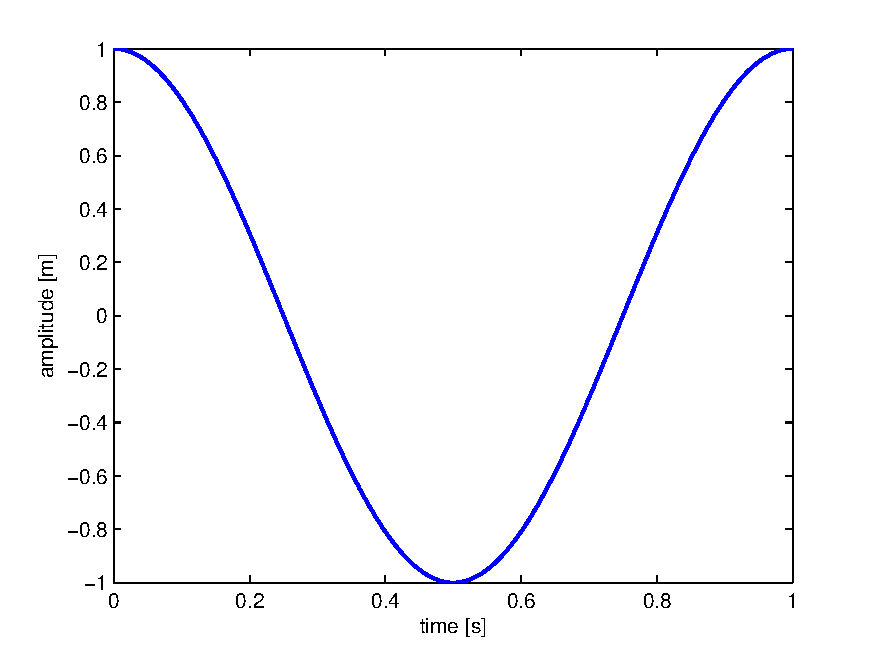
\includegraphics[width=\linewidth]{results}
\caption{In-text Picture}
\label{fig:results}
\end{figure}

Reference to Figure \ref{fig:results}.

\section*{Results and Discussion}

\lipsum[10] % Dummy text

\subsection*{Subsection}

\lipsum[11] % Dummy text

\subsubsection*{Subsubsection}

\lipsum[12] % Dummy text

\subsubsection*{Subsubsection}

\lipsum[14] % Dummy text

\subsection*{Subsection}

\lipsum[15-20] % Dummy text

\section*{Acknowledgments}

So long and thanks for all the fish.

\bibliography{thesis}

\end{document}
